
\section{Introduction}

In this chapter,  we explore global-in-time or finite-horizon optimization. The objective is to maximize mixing  at a prescribed final time as oppose to instantaneously as before.  This optimization problem employs the techniques from calculus of variations and optimal control \cite{Kirk2004a, gelfand2000calculus, fox1950introduction,troltzsch2010optimal, bertsekas1995dynamic,liberzon2011calculus}. We will focus primarily on the enstrophy-constrained case but will explicitly mention when analogous results carry over to the energy-constrained problem.

This chapter is organized as follows. We introduce the theory and setup of the optimization problem in Section \ref{sec:git_theory}. This section introduces the associated Euler-Lagrange equations and total variation. Section \ref{sec:numerical_method} describes two numerical methods for solving the Euler-Lagrange equations. Lastly, analytical and numerical results are presented in Section \ref{sec:git_results} for the pure advective case ($\kappa = 0$).

This project is currently ongoing and the work done so far is presented. 
\section{Theory}
\label{sec:git_theory}
\subsection{The optimal control problem}
Here we describe the global-in-time optimization problem for enstrophy-constrained flows. Let $D=[0,L]^{d}$ be our domain where $L$ is the side length and $d$ is the total number of spatial dimensions. All functions defined on $D$ have periodic boundary conditions. We are interested in the following optimization problem:
\begin{equation}
	\label{eq:PDE_GIT}
	\min_{\mathbf{u}} \|\theta(\,\cdot\,,T)\|_{H^{-1}}^{2}
\end{equation}
subject to the constraints
\begin{equation}
	\label{eq:PDE_advection2-git}
	\partial_{t}\theta+\mathbf{u}\cdot \nabla \theta= \kappa \Delta \theta
\end{equation}
with 
\begin{equation}
\label{eq:PDE_divfree2-git}
\nabla \cdot \mathbf{u} = 0
\end{equation}
and a {\it time-averaged} enstrophy constraint
\begin{equation}
	\label{eq:PDE_enstrophy-git}
	\frac{1}{T}\int_{0}^{T}\int d^{d}x dt |\nabla\mathbf{u}|^{2} = \Gamma^2 L^{d}.
\end{equation}
In addition, we are provided with initial data
\begin{equation}
	\label{eq:PDE_initial_condition2-git}
	\theta(\mathbf{x},0)=\theta_{0}(\mathbf{x}).
\end{equation}
%
\subsection{First and total variation for enstrophy-constraint}

Calculus of variations provides the appropriate framework for investigating the conditions placed on optimizers of functionals. Here we present the first and total variation results for the enstrophy-constrained case with diffusion. Prior to presenting these results, it is useful to make the following definitions:

\begin{itemize}
\vspace{0.25 cm}

\item \noindent \textbf{Definition} The pair of functions $\{\theta^{*}(x,t), \mathbf{u}^{*}(x,t)\}$ on $D$ is said to be \textbf{admissible} if it satisfies the following constraints \[\partial_{t}\theta+\vec{u}\cdot \nabla \theta=\kappa \Delta \theta \]
\[\nabla\cdot \mathbf{u}=0\]
\[\int_{0}^{T}\int_{D}d^{d}xdt |\nabla \mathbf{u}|^{2}=\Gamma^2L^{d}T\] and the initial data $\theta(\mathbf{x},0)=\theta_{0}(\mathbf{x})$.

\vspace{0.25 cm}

\item \noindent \textbf{Definition} An admissible pair $\{\theta^{*}(\mathbf{x},t), \mathbf{u}^{*}(\mathbf{x},t)\}$ on $D$ is said to be an \textbf{optimal solution}, \textbf{minimizer}, or \textbf{minima} of the cost functional $C$ if the \textbf{total variation}
\[\Delta C=C\{\theta, u \}-C\{\theta^{*},u^*\} \] is non-negative for all admissible pairs $\{\theta,\mathbf{u}\}$.

\vspace{0.25 cm}

\noindent

\item \noindent \textbf{Definition} A pair $\{\theta(\mathbf{x},t), \mathbf{u}(\mathbf{x},t)\}$ on $D$ is said to be an \textbf{extrema} for the cost functional $C$ if the pair is admissible and the \textbf{first variation}
\[\delta C=\lim_{\epsilon\rightarrow0}\frac{C\{\theta+\epsilon\tilde{\theta},\mathbf{u} + \epsilon\tilde{ \mathbf{u}}\}-C\{\theta,\mathbf{u}\}}{\epsilon} \] vanishes.
\end{itemize}


It remains to be shown that a minimizer exists within the constrained set of velocity fields satisfying incompressibility and in the $H^1$ Sobolev space (required by the enstrophy constraint).  Is this a sufficient restriction to ensure that a minimizer exists? Proving the existence of a minimizer typically requires demonstrating weakly lower semicontinuity of the cost functional for a sufficiently restricted set of velocity fields. Furthermore, it remains to be shown that a minimizer is an extrema and thus must satisfy the Euler-Lagrange equations which require sufficient regularity of the cost functional. In the context of traditional calculus, this is analogous to ensuring that a minimizer of a function coincides with a point where the derivative is zero. Nevertheless, it is still worthwhile to solve the Euler-Lagrange equations for candidate solutions. To determine the Euler-Lagrange equations, we introduce the associated augmented Lagrangian
\begin{multline}
	\label{eq:PDE_lagrangian}
	\mathcal{L} = \frac{1}{2}\int_{D}d^{d}x |\nabla\Delta^{-1} \theta(\mathbf{x},T)|^{2}  +  \int_{D}d^{d}x \phi_0 (\theta(\mathbf{x},0)-\theta_0(\mathbf{x})) \\
	+ \int_{D} d^{d}x \int dt \left\{ \phi(\partial_{t}\theta+\mathbf{u}\cdot\nabla \theta - \kappa\Delta \theta) +\frac{\mu}{2} (|\nabla \times\mathbf{u}|^{2}- \Gamma^2) + p(\nabla\cdot \mathbf{u})
	\right \} 
\end{multline}
where $\phi_0, \phi, \mu, $ and $p$ are Lagrange multipliers introduced to enforce the system constraints. Assuming that a minimizer is an extrema, we find that a minimizer must satisfy the Euler-Lagrange equations:
\begin{subequations}
\label{eq:pde_first_variation_enstrophy}
\begin{equation}
	\label{eq:PDE_first_variation_1} 
	\frac{\delta \mathcal{L}}{\delta \theta(T)}=0 \quad \Rightarrow  \quad \Delta^{-1} \theta(\mathbf{x},T) - \phi(\mathbf{x},T) = 0 
\end{equation}
\begin{equation}
	\frac{\delta \mathcal{L}}{\delta \theta}=0 \quad \Rightarrow \quad\partial_{t}\phi + \mathbf{u}\cdot\nabla\phi   + \kappa \Delta \phi =0
	\label{eq:PDE_first_variation_2} 
\end{equation}
\begin{equation}
	\frac{\delta \mathcal{L}}{\delta  u}=0  \quad \Rightarrow  \quad   \phi \nabla\theta - \nabla p -\mu \Delta \mathbf{u}=0. \label{eq:PDE_first_variation_3}
\end{equation}
\begin{equation}
	\label{eq:PDE_first_variation_4}
	\frac{\delta \mathcal{L}}{\delta \phi}=0  \quad \Rightarrow  \quad  \partial_{t}\theta+\mathbf{u}\cdot \nabla \theta - \kappa \Delta \theta = 0
\end{equation}
\begin{equation}
\label{eq:PDE_first_variation_5}
\frac{\delta \mathcal{L}}{\delta p}=0 \quad \Rightarrow  \quad  \nabla \cdot \mathbf{u} = 0
\end{equation}
\begin{equation}
	\label{eq:PDE_first_variation_6}
\frac{\delta \mathcal{L}}{\delta \mu}=0 \quad \Rightarrow  \quad 	\int_{0}^{T}\int d^{d}x dt |\nabla \times \mathbf{u}|^{2} - \Gamma^2 L^{d}T = 0
\end{equation}
\begin{equation}
	\label{eq:PDE_first_variation_7}
\frac{\delta \mathcal{L}}{\delta \phi_0}=0 \quad \Rightarrow  \quad	\theta(\mathbf{x},0) - \theta_{0}(\mathbf{x}) = 0.
\end{equation}
\end{subequations}
Note that equation \ref{eq:PDE_first_variation_2} has the same analytic and numerical challenges as the backwards heat equation given the sign of diffusion term. As a consequence, this equation will be solved backwards in time in our numerical schemes presented in a later section.

%\subsubsection{Second and Total Variation}
%
%\begin{flushleft}
%
%Let $\theta(\mathbf{x},t)$ and $\mathbf{u}(\mathbf{x},t)$ be arbitrary functions on $D \times [0,T]$ and define a cost functional be
%\[
%C\{\theta\}=\| \theta(\mathbf{x},T)\|^{2}_{H^{-1}}=\int_{D}d\mathbf{x} |\nabla^{-1} \theta(\mathbf{x},T)|^{2}.\]
%
%Define the quantities:
%\begin{align*}
%g_{1}\{\theta,\mathbf{u}\} &= \partial_{t}\theta+\mathbf{u}\cdot \nabla \theta - \kappa \Delta \theta \\
%g_{2}\{\mathbf{u}\} &= \nabla\cdot \mathbf{u} \\
%g_{3}\{\mathbf{u}\} &= \int_{0}^{T}\int_{D}d\mathbf{x}dt |\nabla \mathbf{u}|^{2}-TL^{d}\Omega^{2}.
%\end{align*}
%
%Let $\phi(\mathbf{x},t),$ and $ q(\mathbf{x},t)$ be arbitrary functions on $D \times [0,T]$ and let $\mu$ be a scalar. Define the functional $G$ as
%
%\begin{equation}
%\label{eq:constraint-functional}
%G\{\theta,\mathbf{u},\phi,q,\mu\}=\iint [\phi(\mathbf{x},t) g_{1}\{\theta,\mathbf{u}\} + q(\mathbf{x},t) g_{2}\{\mathbf{u}\}]d\mathbf{x}dt+\mu g_{3}\{\mathbf{u}\}
%\end{equation}
%
%Let the pair $\{\theta_{0},\mathbf{u}_{0}\}$ be an extrema of $C$ and $\{\theta_{1},\mathbf{u}_{1}\}$ be an admissible pair. Note that since $\{\theta_{0},\mathbf{u}_{0}\}$ and $\{\theta_{1},\mathbf{u}_{1}\}$ are admissible, $G\{\theta_{0},\mathbf{u}_{0},\phi,q,\mu\}=0$ and $G\{\theta_{1},\mathbf{u}_{1},\phi,q,\mu\}=0$. Hence, the total variation of G is also zero,
%\[\Delta G= G\{\theta_{1},\mathbf{u}_{1},\phi,q,\mu\}-G\{\theta_{0},\mathbf{u}_{0},\phi,q,\mu\}=0.\]
%
%
% Let $\delta\theta=\theta_{1}-\theta_{0}$ and $\delta \mathbf{u}=\mathbf{u}_{1}-\mathbf{u}_{0}$.
% 
% \[\Delta G=\iint [\phi(\mathbf{x},t) g_{1}\{\theta_{1},\mathbf{u}_{1}\} + q(\mathbf{x},t) g_{2}\{\mathbf{u}_{1}\}]d\mathbf{x}dt+\mu g_{3}\{\mathbf{u}_{1}\}\]
%  \[-\iint [\phi(\mathbf{x},t) g_{1}\{\theta_{0},\mathbf{u}_{0}\} + q(\mathbf{x},t) g_{2}\{\mathbf{u}_{0}\}]d\mathbf{x}dt-\mu g_{3}\{\mathbf{u}_{0}\}\]
%  
%  \begin{eqnarray*}
% 	 &=& \iint [
%  		\phi\left(
%  			\partial_{t}(\theta_{0}+\delta\theta)+(\mathbf{u}_{0}+\delta\mathbf{u})\cdot \nabla(\theta_{0}+\delta\theta)
%  			-\partial_{t}\theta_{0}-\mathbf{u}_{0}\cdot \nabla 					\theta_{0}
%	  	\right) \\
%	&+& q\left(
%		\nabla\cdot(\mathbf{u}_{0}+\delta\mathbf{u})-\nabla\cdot\mathbf{u_{0}}	
%	  	\right) \\
%	&+&\mu \left( 
%		 	 |\nabla(\mathbf{u}_{0}+\delta\mathbf{u})|^{2}- |\nabla \mathbf{u}_{0}|^{2}
%	  	\right)
%  ]d\mathbf{x}dt
%\end{eqnarray*}
%
%  \begin{eqnarray*}
% 	\implies \Delta G &=& \iint \{
%  		(-\partial_{t}\phi-\mathbf{u}_{0}\cdot\nabla\phi)\delta\theta
%		+( \phi \nabla\theta_{0} - \nabla q -\mu \Delta \mathbf{u}_{0})\cdot \delta\mathbf{u} \\
%		 &+&\nabla\phi\cdot\delta\mathbf{u}\delta \theta 
%		 +\mu |\nabla\delta \mathbf{u}|^{2}  
%  		t\}d\mathbf{x}dt \\
%  &+& \int_{D}\phi(x,T)\delta\theta(x,T)d\mathbf{x} = 0
%\end{eqnarray*}
% 
%  
% 
%  Consider the total variation of C
% \[ \Delta C= C\{\theta_{1}\}-C\{\theta_{0}\} \] 
% \[=\int_{D}\left\{ |\nabla^{-1}\theta_{1}(\mathbf{x},T)|^{2} - |\nabla^{-1} \theta_{0}(\mathbf{x},T)|^{2} \right\} d\mathbf{x} \]
% 
%\[=\int_{D}\left\{ 
%  			|\nabla^{-1} \left[
%  				\theta_{0}(\mathbf{x},T)+\delta\theta(\mathbf{x},T)											\right]|^{2} 
%  			- |\nabla^{-1} \theta_{0}(\mathbf{x},T)|^{2} 
%  		\right\} 
%d\mathbf{x} \]
%  
%\[
%	=\int_{D}
%	\left\{ 
%   		\nabla^{-1}\theta_{0}(\mathbf{x},T)\cdot
%   		\nabla^{-1} \delta\theta(\mathbf{x},T)
%   		+|\nabla^{-1} 
%		\delta\theta(\mathbf{x},T)|^{2} 
%   \right\} 
%   d\mathbf{x}  
%\]
% 
%\[
%	=\int_{D}
%	\left\{ 
%   		-\Delta^{-1}\theta_{0}(\mathbf{x},T)\delta\theta(\mathbf{x},T)
%   		+|\nabla^{-1} 
%		\delta\theta(\mathbf{x},T)|^{2} 
%   \right\} 
%   d\mathbf{x}  
%\]
% 
%Since $\Delta G=0$, we can add  $\Delta G$ to $\Delta C$ without any consequence. Let the index ``$_{T}$'' be shorthand for the arguments $(\mathbf{x},T)$. (e.g. $\phi_{T}=\phi(\mathbf{x},T)$)
%
%
%  \begin{eqnarray*}
% 	\Delta C&=& \Delta C+\Delta G \\
% 	         &=& \iint \left\{
%  			(-\partial_{t}\phi-\mathbf{u}_{0}\cdot\nabla\phi)\delta\theta
%			+( \phi \nabla\theta_{0} - \nabla q -\mu \Delta \mathbf{u}_{0})\cdot \delta\mathbf{u}
%			 +\nabla\phi\cdot\delta\mathbf{u}\delta \theta 
%			 +\mu |\nabla\delta \mathbf{u}|^{2}  
%  		\right\}d\mathbf{x}dt \\
%		  &+& \int_{D}\left\{
%  			(\phi_{T}-\Delta^{-1}\theta_{0,T})\delta\theta_{T}
%   			+|\nabla^{-1} 
%			\delta\theta_{T}|^{2}
%	       \right\} d\mathbf{x}		
%\end{eqnarray*}
% 
%
%Assuming that the global optimizer has vanishing first variation, we must show that the second variation (all quadratic terms of perturbations) is nonnegative for a candidate global minimum. For the moment suppose that the first variation vanishes, then 

We highlight that \ref{eq:pde_first_variation_enstrophy} provides necessary, but not sufficient, conditions for an optimal solution. To prove optimality, it suffices to show the total variation at an extrema (see Appendix \ref{sec:variation_calc} for calculation details)
  \begin{eqnarray}
  	\label{eq:total_Variation}
 	\Delta C&=& \iint \left\{\nabla\phi\cdot\delta\mathbf{u}\delta \theta 
			 +\mu |\nabla\delta \mathbf{u}|^{2}  
  		\right\}d\mathbf{x}dt +\int_{D}
  			|\nabla^{-1} 
			\delta\theta_{T}|^{2}
	      d\mathbf{x} \geq 0
\end{eqnarray}
%
for all perturbations $\delta\theta = \tilde{\theta}-\theta$ and $\delta \mathbf{u} = \tilde{\mathbf{u}}-\mathbf{u}$ about the candidate solution $\{\theta,\mathbf{u}\}$ where $\{\tilde{\theta},\tilde{\mathbf{u}}\}$ is admissible. That said, this is a non-convex optimization problem so this is not a trivial task.

%\end{flushleft}

\subsection{First and total variation for energy constraint}
The analysis for the energy-constrained problem with $\frac{1}{T}\int_{0}^T\ltwo{\mathbf{u}}^2 = U^2L^2$ is similar to that for the enstrophy-constrained problem. Here we simply state the analogous results. The augmented Lagrangian for energy constrained problem is 
\begin{multline}
	\label{eq:PDE_lagrangian}
	\mathcal{L} = \frac{1}{2}\int_{D}d^{d}x |\nabla\Delta^{-1} \theta(\mathbf{x},T)|^{2}  +  \int_{D}d^{d}x \phi_0 (\theta(\mathbf{x},0)-\theta_0(\mathbf{x})) \\
	+ \int_{D} d^{d}x \int dt \left\{ \phi(\partial_{t}\theta+\mathbf{u}\cdot\nabla \theta ) +\frac{\mu}{2} (|\mathbf{u}|^{2}- U^2) + p(\nabla\cdot \mathbf{u})
	\right \} .
\end{multline}
%
The Euler-Lagrange equations are
\begin{subequations}
\begin{equation}
	\label{eq:PDE_first_variation_1_energy} 
	\frac{\delta \mathcal{L}}{\delta \theta(T)}=0 \quad \Rightarrow  \quad \Delta^{-1} \theta(\mathbf{x},T) - \phi(\mathbf{x},T) = 0 
\end{equation}
\begin{equation}
	\frac{\delta \mathcal{L}}{\delta \theta}=0 \quad \Rightarrow \quad\partial_{t}\phi + \mathbf{u}\cdot\nabla\phi   + \kappa \Delta \phi =0
	\label{eq:PDE_first_variation_2_energy} 
\end{equation}
\begin{equation}
	\frac{\delta \mathcal{L}}{\delta  u}=0  \quad \Rightarrow  \quad   \phi \nabla\theta - \nabla p +\mu \mathbf{u}=0. \label{eq:PDE_first_variation_3_energy}
\end{equation}
\begin{equation}
	\label{eq:PDE_first_variation_4_energy}
	\frac{\delta \mathcal{L}}{\delta \phi}=0  \quad \Rightarrow  \quad  \partial_{t}\theta+\mathbf{u}\cdot \nabla \theta - \kappa \Delta \theta = 0
\end{equation}
\begin{equation}
\label{eq:PDE_first_variation_5_energy}
\frac{\delta \mathcal{L}}{\delta p}=0 \quad \Rightarrow  \quad  \nabla \cdot \mathbf{u} = 0
\end{equation}
\begin{equation}
	\label{eq:PDE_first_variation_6_energy}
\frac{\delta \mathcal{L}}{\delta \mu}=0 \quad \Rightarrow  \quad 	\int_{0}^{T}\int d^{d}x dt |\mathbf{u}|^{2} - U^2 L^{d}T = 0
\end{equation}
\begin{equation}
	\label{eq:PDE_first_variation_7_energy}
\frac{\delta \mathcal{L}}{\delta \phi_0}=0 \quad \Rightarrow  \quad	\theta(\mathbf{x},0) - \theta_{0}(\mathbf{x}) = 0
\end{equation}
\end{subequations}
%
and the total variation at an extrema is 
  \begin{eqnarray}
  	\label{eq:total_Variation_energy}
 	\Delta C&=& \iint \left\{\nabla\phi\cdot\delta\mathbf{u}\delta \theta 
			 +\mu |\delta \mathbf{u}|^{2}  
  		\right\}d\mathbf{x}dt +\int_{D}
  			|\nabla^{-1} 
			\delta\theta_{T}|^{2}
	      d\mathbf{x}
\end{eqnarray}
for all perturbations $\delta\theta = \tilde{\theta}-\theta$ and $\delta \mathbf{u} = \tilde{\mathbf{u}}-\mathbf{u}$ about the candidate solution $\{\theta,\mathbf{u}\}$ where $\{\tilde{\theta},\tilde{\mathbf{u}}\}$ is admissible. 
%
\subsection{Optimal control problem with inequality constraints}
One may be interested in the following {\it inequality} constraint on $\mathbf{u}$ in place of equations \eqref{eq:PDE_enstrophy-git}:
%
\begin{equation}
	\label{eq:PDE_enstrophy-git-ineq}
	\int_{0}^{T}\int d^{d}x dt |\nabla \times \mathbf{u}|^{2} \leq \Gamma^2 L^{d}T
\end{equation}
%
This formulation allows for the possibility of not consuming the entire stirring budget. Intuitively, this seems an unlikely scenario since it seems inefficient not to use of one's stirring resources. We provide the following argument that the inequality constraint is likely saturated for $\kappa = 0$ but not necessarily for $\kappa \neq 0$.

Consider the enstrophy constraint with $\kappa = 0$. Suppose $\{\theta^{*}, u^{*}\}$ are minima where \eqref{eq:PDE_enstrophy-git-ineq} is not saturated and $\int_{0}^{T}\int d^{d}x dt |\nabla \times \mathbf{u}|^{2} = m \Gamma^2 L^{d}T$ with $0\leq m <1$. Then one can construct new variables $\tilde{\theta},\tilde{\mathbf{u}}$ as  $\tilde{\theta}(\mathbf{x},t) = \theta^{*}(\mathbf{x},ct)$ and $\tilde{\mathbf{u}}(\mathbf{x},t) =c u^{*}(\mathbf{x},ct)$ defined for $t\in [0,T/c]$.  Any intermediate $c$ ($1< c < \frac{1}{m}$) will produce the original final-time mix-norm value but at an earlier time $t= T/c$ with available budget $(1-c^2m^2)\Gamma^2L^dT$ left over. Therefore, if there exists {\it any} $\mathbf{u}$ defined for the remaining time ($t\in [T/c,T]$) that is able to decrease the mix-norm by even the slightest amount with budget remaining, then this new candidate solution ($\tilde{\mathbf{u}}$ for $t\in [0,T/c]$ and  $\mathbf{u}$ for $t\in [T/c,T]$) defeats the supposed minima $\{\theta^{*}, \mathbf{u}^{*}\}$.  The instantaneous optimal strategy from the previous chapter is a good candidate, however there are cases where the first derivative of the mix-norm can not be controlled. This case must be dealt with to make this argument rigorous. 

Nevertheless, it still remains worthwhile to formulate the inequality-constrained optimal control problem. We may have confidence that the bound is saturated in the $\kappa =0$ case (given the argument above), but it not obvious that it will always be saturated with diffusion. In fact, there are trivial cases where $\mathbf{u} = 0$ is a reasonable choice. Consider the enstrophy case with initial data $\theta(\mathbf{x},0)$ given by a Fourier mode with large wavenumber $k_0$ and with a corresponding wavelength that is much smaller than the Batchelor wavenumber $k_{B} = \sqrt{\Gamma/\kappa}$. If $\mathbf{u} = 0$, then the advection-diffusion equation becomes simply the diffusion equation, and the mix-norm exhibits exponential decay with rate $-\kappa k_0^2$. However from the local-in-time optimization study of the previous chapter, we found that when advection and diffusion are both actively attempting to minimize the mix-norm, the scalar field develops length scales comparable to the Batchelor scale in the long run. Therefore, a rough approximation of the long-term exponential rate is likely to be $-\kappa k_{B}^2 = -\Gamma$. Therefore in the case were $\Gamma < \kappa k_0^2$, then $\mathbf{u} = 0$ may be a reasonable choice. In other words, stirring (when $\mathbf{u}\neq 0$) may move some spectral mass to wave numbers less than the Batchelor wavenumber and be disruptive. This argument gives reason to believe that the optimal strategy may not always benefit from saturation of the budget.


%\subsubsection{Calculus of variations}
%
% We generalize the results of \cite{Forster1978} here.
 
 

%\subsection{Hamiltonian formulation}
%
%
%
%\subsection{Finite-dimensional forms of optimization problem}
%
%The optimization problem of the previous section can be viewed as optimization of a cost with control of an infinite dimensional vector (a function). In practice, it is worthwhile to consider finite forms of the optimization problem presented since the optimization problem will inevitably be solved in this form on a computer. 
%
%In addition, we will gain value by applicability of Hamiton-Jacobi-Bellmann equation and Dynamic Programming.  We will demonstrate that even in the finite dimensional setting the full Dynamic Programming task is still challenging. There are only a select set of examples where the Hamilton-Jacobi-Bellman equation can be solved exactly (such as in the canonical linear-quadratic regulator problem). Its analog in the original problem (if it can even be well-posed) would be an even more challenging task since the analog of the Hamilton-Jacobi-Bellman equation would likely take the form of a variational equation with a functional as a solution. 
%
%The full Hamilton-Jacobi-Bellman equation in the finite form in most cases suffers from the `curse of dimensionality'. Fortunately, there are approximation methods --- the field exploring these methods is known as Approximate Dynamic Programming (also known as Neurodynamic programing and Reinforcement Learning). We will explore these in later sections.
%
%There are two paths to finite-dimensionality reduction: one could optimize first and then reduce or reduce first and then optimize. We will first consider the latter. By optimize, I mean derive the necessary Euler-Lagrange equations. This was done in the previous section. The next step would be to then reduce the dimensionality of these equations in space and time. We will do this step in sequence by first looking at the consequence of reductions in space. 
%
%
%The spatial dimensionality reduction is done by a spectral decomposition into Fourier modes (an appropriate choice due to periodic conditions). The state equation (advection-diffusion equation) in Fourier space is expressed as 
%\begin{equation}
%\label{eq:advection_spectral}
%\partial_{t}\hat{\theta}(\mathbf{k},t)+i\sum_{\mathbf{k}'}\hat{u}(\mathbf{k}-\mathbf{k}',t)\cdot \mathbf{k}' \hat{\theta}(\mathbf{k}',t)+\kappa |\mathbf{k}|^2\theta(\mathbf{k},t)=0
%\end{equation}
%or 
%\begin{equation}
%\label{eq:advection_spectral_condensed}
%\partial_{t}\hat{\theta}(\mathbf{k},t)=i\sum_{\mathbf{k}'}A_{\mathbf{k},\mathbf{k}'} \hat{\theta}(\mathbf{k}',t)-\kappa |\mathbf{k}|^2\theta(\mathbf{k},t)
%\end{equation}
%where 
%\begin{equation}
%A_{\mathbf{k},\mathbf{k}'}=-\hat{u}(\mathbf{k}-\mathbf{k}',t)\cdot \mathbf{k}'.
%\end{equation}
%One can show that $A$ is hermitian ($A=A^{\dagger}$). Note that the above representation is {\it exact} as an infinite system of ordinary differential equations --- no dimensionality reduction so far. Letting $M = K^{-1}K^{-1}$, $K_{\mathbf{k},\mathbf{k}'} = \mathbf{k} \mathds{1}_{\mathbf{k}=\mathbf{k}'}, A = \sum_{\mathbf{k}} \mathbf{\hat{u}}(\mathbf{k}) B(\mathbf{k})$, and $B(\mathbf{k}'')_{\mathbf{k},\mathbf{k}'} = -i\mathbf{k}'\mathds{1}_{\mathbf{k}''=\mathbf{k}'-\mathbf{k}}$, we can write can write the spectral version of the Euler-Lagrange equations as (in matrix form)
%\begin{subequations}
%	\begin{align}
%	\label{eq:matrix_terminal-git}
%	 M\theta(T) - \phi(T) = 0 \\
%	 \label{eq:matrix_adj-git}
%	 \dot{\phi} - A\phi - \kappa K^2\phi= 0	\\
%	 \label{eq:matrix_state-git}
%	 \dot{\theta} - A\theta  - \kappa K^2\theta = 0	\\
%	 \label{eq:matrix_opt-git}
%	 \phi^{T}B(\mathbf{k})\theta + \mu |\mathbf{k}|^2 u(\mathbf{k}) = 0 \\
%	 \frac{1}{T}\int_{0}^T (u^{T}K^{2}u - \Gamma) = 0 \\
%	 \mathbf{k} \cdot u(\mathbf{k}) = 0
%	\end{align}
%	\label{eq:spectral_euler_lagrange}
%\end{subequations}
%where the hatted and bold face has been removed for the state $\theta$, adjoint $\phi$,  and control variables $u$ for clarity. 
%
%Now the discretized system simply follows as a Galerkin truncation of the spectral Euler-Lagrange equations \eqref{eq:spectral_euler_lagrange} above. We choose the truncation where all spectral components with $\|\mathbf{k}\|_{\infty} \leq a $ are kept with a corresponding number $N$ of total Fourier modes in each spatial dimension. Thus giving a total of $N^d$ fourier modes for $d$ spatial dimensions. This will cause a reduction of the matrices $M$, $K$, and $B$ above. Also $A$ becomes  $A = \sum_{\|\mathbf{k}\|_{\infty} \leq a} \mathbf{\hat{u}}(\mathbf{k}) B(\mathbf{k}).$
%
%
%Let's consider the other route to discretization mentioned earlier where we discretize first and then optimize. If we start with the spectral representation as our starting point, the truncation of the state equation and constraints lead to exactly the same expressions derived by the first approach. What remains are the associated equations governing the Lagrange multipliers. To determine these remaining relations, we must find the first variations of the following augmented Lagrangian
%\begin{multline*}
%	\mathcal{ L} \{ \theta, u,\phi,\mu \} = \frac{1}{2} \sum_{\|\mathbf{k}\|_{\infty}<a}^{}\frac{|\theta_{\mathbf{k}}(T)|^2}{|\mathbf{k}|^2} + \int_{0}^{T}\Bigg \{\sum_{\|\mathbf{k}\|_{\infty}<a}^{}\phi_{\mathbf{k}}(t)\left( \dot{\theta} - A\theta  - \kappa K^2\theta \right)_{\mathbf{k}} \\
%	\sum_{\|\mathbf{k}\|_{\infty}<a}q_{\mathbf{k}}(t)\mathbf{k} \cdot u(\mathbf{k}) +  \frac{\mu }{2}\left( u^{T}K^{2}u - \Gamma\right)  \Bigg\}\: dt
%\end{multline*}
%
%We find that the first variation of the above augmented lagrangian results in an identical set of equations derived in the first approach.
%
%We have however, only dealt with the reduction of the systems spatially. To also discretize in time, we have a choice of many numerical integration schemes. We will consider only 1-step numerical schemes of the form: $\theta^{m+1} = f(\theta^{m},u^{m})$ for $m = 1,2, \dots, M $.
%

\section{Numerical method for pure advection ($\kappa = 0$)}
\label{sec:numerical_method}

\subsection{Gradient descent algorithm}
%We perform the following update to $u$ by a conjugate-gradient scheme. At each time step $i$, the preconditioned gradient is given by  $\nabla_{u} J = - (\tilde{u}^{i} - u^{i})$ where $\tilde{u}^{i}$ solves the optimality condition \eqref{eq:matrix_opt-git} after integrating the state equation \eqref{eq:matrix_state-git} forward in time to find $\theta^{i}$ and adjoint equation  \eqref{eq:matrix_adj-git}  backwards in time to find $\phi^{i}$ with using the terminal condition \eqref{eq:matrix_terminal-git}. 
%

Here we describe a numerical method for solving the Euler-Lagrange equations \eqref{eq:PDE_first_variation_1} -- \eqref{eq:PDE_first_variation_7} corresponding the enstrophy-contained problem in 2 dimensions. We use a gradient-based method with line search. The overall strategy is to solve \eqref{eq:PDE_first_variation_1} -- \eqref{eq:PDE_first_variation_7} per iteration except \eqref{eq:PDE_first_variation_3}. The left hand side of \eqref{eq:PDE_first_variation_3} is in fact the gradient of the cost with respect to the velocity field over space and time that is valuable for our iterative update scheme on $\mathbf{u}$. To see that this is the gradient, consider the first variation of the entire augmented functional. If all first variations vanish except the variation with respect to $\mathbf{u}$, then
%
  \begin{eqnarray*}
 	\delta \mathcal{L}&=&  \iint ( \phi \nabla\theta - \nabla p -\mu \Delta \mathbf{u})\cdot \delta\mathbf{u} \,\, d\mathbf{x}dt .
\end{eqnarray*}
%
If in addition ${\theta + \delta\theta,u+ \delta u}$  remains admissible, then 
\begin{equation}
\label{eq:gradient-relation}
\frac{\delta C}{\delta \mathbf{u}} = \frac{\delta L}{\delta \mathbf{u}}=  \phi \nabla\theta - \nabla p -\mu \Delta \mathbf{u}
\end{equation}
for variations respecting the constraints. 

We discretize space as an $N$ by $N$ grid and time from $0$ to $T$ uniformly with $M$ time points. Thus, $\mathbf{u}$ is an array of shape $(M,2,N,N)$. $\theta$ and $\phi$ are arrays of shape $(M,N,N)$. The approach requires satisfying all the Euler-Lagrange equations except \eqref{eq:PDE_first_variation_3} per iteration. The update is of the following form:
\begin{equation}
\label{eq:update}
\mathbf{u}^{k+1} = \mathds{N}\left(\mathbf{u}^{k} - \eta \frac{\delta C}{\delta \mathbf{u}}(\mathbf{u}^{k})\right).
\end{equation}
where $\eta$ is the step size. Note that this updates the velocity field at all points of space and time. $\mathds{N}(\mathbf{v})$ enforces the enstrophy constraint: it is defined as $\mathds{N}(\mathbf{v}) = \alpha \mathbf{v}$ where $\alpha$ is a normalizing factor and chosen so $\frac{1}{T}\int_0^Tdt\|\nabla \mathds{N}(\mathbf{v}) (\,\cdot\, ,t)\|_{2}^2 = \Gamma^2 L^2 $.

To calculate $\frac{\delta C}{\delta \mathbf{u}}(\mathbf{u}^{k}) =  \phi^{k} \nabla\theta^{k} - \nabla p^{k} -\mu^{k} \Delta \mathbf{u}^{k}$, we must find $\theta^{k}, \phi^{k},\mu^{k}$ and $p^{k}$. $\theta^{k}$ is determined at each iteration from $\mathbf{u}^{k}$ by integrating the advection-diffusion equation with initial condition $\theta_0$. Then the terminal condition $\phi^{k}(\mathbf{x},T) = \Delta^{-1} \theta^{k}(\mathbf{x},T)$ is used to provide an `initial condition' for $\phi^{k}$. The velocity $\mathbf{u}^{k}$ is used to evolve adjoint equation for $\phi^{k}$ backwards in time given $\phi^{k}(\mathbf{x},T).$ Both integrations forward and backwards in time are done with a Fourier basis with $N$ modes to represent the spatial domain and a 2nd order Heun's time-stepping method. $N$ is chosen sufficiently large to to resolve spatially for all time. $dt $ is chosen small enough to satisfy both advective and diffusive CFL conditions. This criteria is compactly stated as $dt=0.25\min[1/(\Gamma N),L^2/(\kappa N^2)]$.  If we demand that the updated $\mathbf{u}^{k+1}$ be incompressible, then this requires that $\frac{\delta C}{\delta \mathbf{u}}(\mathbf{u}^{k})$ be incompressible. Towards this goal, we take the divergence of both sides of \eqref{eq:gradient-relation} and require that it vanish. This gives the following choice of $p^{k} = \Delta^{-1} \nabla \cdot (\phi^k \nabla \theta^k)$ which is equivalent to applying the divergence-free projection operator $\mathds{P}$ to $\frac{\delta C}{\delta \mathbf{u}}(\mathbf{u}^{k})$ where the projector $\mathds{P}(\mathbf{v})$ is defined as $\mathds{P}(\mathbf{v}) = \mathbf{v} - \nabla\Delta^{-1}(\nabla \cdot \mathbf{v})$. Lastly $\mu^{k}$ is chosen so that the update obeys the enstrophy constraint. This restriction is captured in the condition $\int_0^T\int_{D}\Delta \mathbf{u} \cdot \delta \mathbf{u}^k d\mathbf{x}dt= 0$ where $\delta \mathbf{u} = \mathbf{u}^{k+1} - \mathbf{u}^{k}$. According to our update and for small $\delta \mathbf{u}$ or equivalently $\eta$, this is approximately  given by $\delta \mathbf{u} \approx \eta\frac{\delta C}{\delta \mathbf{u}}(\mathbf{u}^{k}).$ We then calculate:
\begin{eqnarray}
\label{eq:linearized_constraint}
0 &=& \int_0^T\int_{D}d\mathbf{x}dt \, \Delta \mathbf{u}^{k} \cdot \delta \mathbf{u} \\
&=& \eta \int_0^T\int_{D}d\mathbf{x}dt \, \Delta \mathbf{u}^k \cdot ( \phi^k \nabla\theta^k- \nabla p^{k} -\mu^{k}\Delta \mathbf{u}^{k}) \\
&=&  \eta \int_0^T\int_{D}d\mathbf{x}dt \, \Delta \mathbf{u}^k \cdot (\mathds{P}(\phi^k \nabla\theta^k) -\mu^{k} \Delta\mathbf{u}^{k}) \\
 \end{eqnarray}
Therefore, we find that 
\begin{equation}
\mu^{k} =\frac{ \int_0^T\int_{D}d\mathbf{x}dt \, \Delta \mathbf{u}^k  \cdot \mathds{P}(\phi^k \nabla\theta^k)}{ \int_0^T\int_{D}d\mathbf{x}dt \, \Delta \mathbf{u}^k  \cdot \Delta \mathbf{u}^k }.
\end{equation}
This choice $\mu^{k}$ is chosen to enforce the enstrophy constraint. Note that \eqref{eq:linearized_constraint} is the {\it linearized} constraint condition. This is why we enforced this constraint by introducing the normalizing operator $\mathds{N}()$. The method as a whole is summarized in Figure \ref{fig:GD-algorithm}.  

We perform the following validation of the gradient by considering its projection onto the search direction $\mathbf{d} = - \frac{\delta C}{\delta \mathbf{u}}$ at $\mathbf{u}$ (chosen to be local-in-time velocity field).  We first computing the directional analytical gradient by 
\begin{equation}
G_{a} =\frac{ \int_0^T\int_{D}d\mathbf{x}dt \, \frac{\delta C}{\delta \mathbf{u}} \cdot \mathbf{d} }{ \int_0^T\int_{D}d\mathbf{x}dt \,  \mathbf{d}\cdot \mathbf{d} }.
\end{equation} 
and the finite-difference approximation with step $\epsilon$ given by 
\begin{equation}
G_{\epsilon} = \frac{C(\mathbf{u} + \epsilon\mathbf{d})- C(\mathbf{u} - \epsilon\mathbf{d})}{2\epsilon}
\end{equation} 
We can then compare the analytic gradient $G_{a}$ and its approximation $G_{\epsilon}$ to find the relative error $R$ defined as 
\begin{equation}
R = \frac{|G_{a}-G_{\epsilon}|}{|G_{a}|} 
\end{equation}
as function of $\epsilon$ as shown in figure \ref{fig:gradient}. Note that we get a decay in the relative error with smaller $\epsilon$ which eventually plateau to $R \approx 10^{-3}$ which is likely due to truncation error associated with our choices of $N$ and $M$. If $N$ and $M$ are increased, we would expect this saturated plateau to decrease. Improvements to determining an accurate gradient will be investigated further since it is important to have an accurate gradient for an efficient gradient descent search.



\begin{figure}

\begin{algorithmic}[1]
\Function{Gradient\_Descent($u_0$,$\theta_0$,\textit{tol})}{}
\State$u$ $\gets$ zeros array of shape (M,2,N,N)
\State $\theta$ $\gets$ zeros array of shape (M,N,N)
\State $\phi$ $\gets$ zeros array of shape (M,N,N)
\State
\State $u[0]$ $\gets$ $u_0$
\State
 \While {$\|\frac{\delta C}{\delta u}\| \geq tol$}
	\State  $\theta$ $\gets$ integrate\_forward($u$ ,$\theta_0$)
	\State  $\phi[M-1]$  $\gets  \Delta^{-1}(\theta[M-1]$)
	\State $\phi$ $\gets$ integrate\_backward($u$ ,$\phi[M-1]$)
	\State
	\State  $\frac{\delta C}{\delta u} \gets$ compute\_gradient($\theta,\phi,u$)
	\State  $d \gets  $divergence\_free\_projection($-\frac{\delta C}{\delta u} $)
	\State $\eta  \gets$ line\_search($u$,$d$)
	\State $u \gets$ normalize($u + \eta d$)
\EndWhile
\State	
\Return $u$
\EndFunction
\end{algorithmic}
\caption{Gradient descent for final-time optimization}
\label{fig:GD-algorithm}
\end{figure}

\begin{figure}
\centering
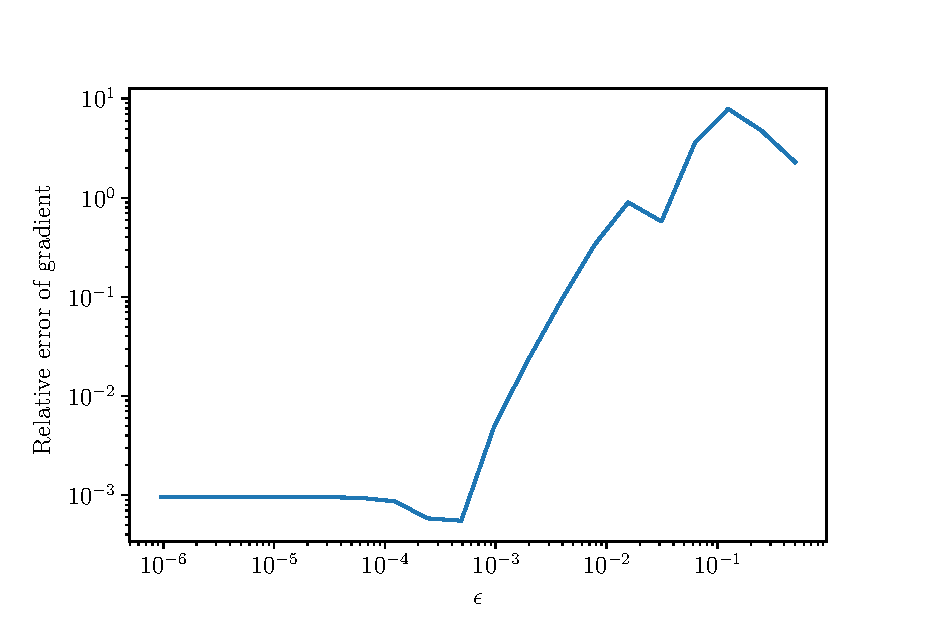
\includegraphics[width=0.7\textwidth]{ch-git/images/gradient}
\caption{The relative numerical error between analytical and finite-difference gradient as a function of the finite-difference step size $\epsilon$.}
\label{fig:gradient}
\end{figure}

\subsection{Target algorithm}
\label{sec:target_method}
The previous gradient descent algorithm picks the search direction $d$ to be proportional to the negative gradient. Here we purpose a different search direction that has improved convergence at least demonstrated in practice for the problem of interest and parameters chosen. The update is
\begin{equation}
\label{eq:target_update}
\mathbf{u}^{k+1} = \mathds{N}(\mathbf{u}^k + \eta \mathbf{d}^k)
\end{equation}
where $\mathbf{d}^k = \mathbf{u}_{t}^k - \mathbf{u}^k$ and $\mathbf{u}_t^k$ is the `target' solution given by 
\begin{equation}
\mathbf{u}_t^k = \mathds{N}(\Delta^{-1} \mathds{P}(\phi^{k} \nabla \theta^{k})).
\end{equation}
$\phi^{k}$ and $\theta^{k}$ are determined by integrating forward and backwards in time with $\mathbf{u}^{k}$ as seen before in the gradient descent algorithm. The above expression can be viewed as the solution to $ \phi^{k} \nabla\theta^{k} - \nabla p^{k} -\mu^{k} \Delta \mathbf{u}^{k}_t= 0$ where the $\mathbf{u}_t^{k}$ takes the place of $\mathbf{u}^{k}$ in the gradient expression while keeping $\theta^k$ and $\phi^{k}$ as solutions to the state and adjoint equations corresponding to $\mathbf{u}^{k}$. $\mu^{k}$ and $p^{k}$ are embodied in the normalization and divergence-free projection operators that require $\mathbf{u}_t^k$ to satisfy incompressibility and the intensity constraint. The algorithm is summarized in figure \ref{fig:target}.

\begin{figure}
\begin{algorithmic}[1]
\Function{Target($u_0$,$\theta_0$,\textit{tol})}{}
\State$u$ $\gets$ zeros array of shape (M,2,N,N)
\State $\theta$ $\gets$ zeros array of shape (M,N,N)
\State $\phi$ $\gets$ zeros array of shape (M,N,N)
\State
\State $u[0]$ $\gets$ $u_0$
\State
 \While {$\|d\| \geq tol$}
	\State  $\theta$ $\gets$ integrate\_forward($u$ ,$\theta_0$)
	\State  $\phi[M-1]$  $\gets  \Delta^{-1}(\theta[M-1]$)
	\State $\phi$ $\gets$ integrate\_backward($u$ ,$\phi[M-1]$)
	\State
	\State  $u_{target} \gets$ compute\_target($\theta,\phi,u$)
	\State  $d \gets  u_{target} - u$
	\State $\eta  \gets$ line\_search($u$,$d$)
	\State $u \gets$ normalize($u + \eta d$)
\EndWhile
\State	
\Return $u$
\EndFunction
\end{algorithmic}
\caption{Target algorithm for final-time optimization}
\label{fig:target}
\end{figure}



%
%\subsection{Hamilton-Jacobi-Bellman equation}
%So far, we have discussed only variational approach to optimal control. Here we introduce a dynamic programming perspective. The Hamilton-Jacobi-Bellman equation is given by 
%
%\begin{equation}
%\frac{\partial}{\partial t} V(\theta,t) = \min_{u}\left\{ \sum_{\mathbf{k}} \frac{\partial V(\theta, t)}{\partial \theta_{\mathbf{k}}} \frac{\partial \theta_{\mathbf{k}}}{\partial t}(\theta, u)\right\}
%\end{equation}
%with terminal condition $V(\theta,T) = \sum_{\mathbf{k}}\frac{|\theta_{\mathbf{k}}|^2}{|\mathbf{k}|^2}$ where $V(\theta,t): \mathds{C}^{N^d} \times [0,T] \rightarrow \mathds{R}$ and .
%
%As an aside, although the summation is over a finite set of $\mathbf{k}$ values, I speculate that the summation could just as well be over an infinite set of $\mathbf{k}$ for the full spectral formulation. In this case, $V$ is now a real-valued mapping over an infinite-dimensional vector space and hence is a functional. 
%
%Returning to the analysis of the reduced system, the time-discretized version is given by 
%\begin{equation}
%V^{n-1} (\theta)= \min_{u^{n-1}}\left\{ \sum_{\mathbf{k}} \frac{\partial V^{n}(\theta)}{\partial \theta_{\mathbf{k}}} f_{\mathbf{k}}(\theta, u)\right\}
%\end{equation}
%
%
%\subsection{Approximate Dynamic Programming}
%% \subsubsection{Instantaneous optimization as a one-step look ahead scheme} 
     
\section{Results for pure advection ($\kappa = 0$)}
\label{sec:git_results}
\subsection{Optimal budget use is uniform in time}
Recall that the velocity field is required to have a fixed {\it mean} enstrophy of $\Gamma$ over time. Surprisingly, we find that it is optimal to expend enstrophy uniformly in time. This is shown by the calculation using the Euler-Lagrange equations:
\begin{align*}
	\frac{d}{dt}\int_{D} d^{d}x | \nabla \times \mathbf{u} |^2 &= -\int_{D} d^{d}x \Delta\frac{\partial\mathbf{u}}{\partial t}\cdot \mathbf{u} \\
	&=- \frac{1}{\mu} \int_{D} d^{d}x \left(\frac{\partial\phi}{\partial t}\nabla \theta +\phi\nabla\frac{\partial\theta}{\partial t}  -\nabla \frac{\partial p}{\partial t} \right)\cdot \mathbf{u} \\
	&=- \frac{1}{\mu} \int_{D} d^{d}x \left(\frac{\partial\phi}{\partial t}\nabla \theta +\phi\nabla\frac{\partial\theta}{\partial t} \right)\cdot \mathbf{u} \\
	&=- \frac{1}{\mu} \int_{D} d^{d}x \left(\frac{\partial\phi}{\partial t}\mathbf{u} \cdot \nabla \theta -\mathbf{u} \cdot \nabla \phi\frac{\partial\theta}{\partial t} \right) \\
	&=0 
\end{align*}
Thus, enstrophy is utilized uniformly in time for a minimizer to problem (\ref{eq:PDE_GIT}) (provided that the minimizer satisfies the Euler-Lagrange equations).  This shows another commonality between the partial differential equation and shell model. A similar calculation reveals that energy is conserved in time for the energy-constrained problem.


\begin{figure}
\centering
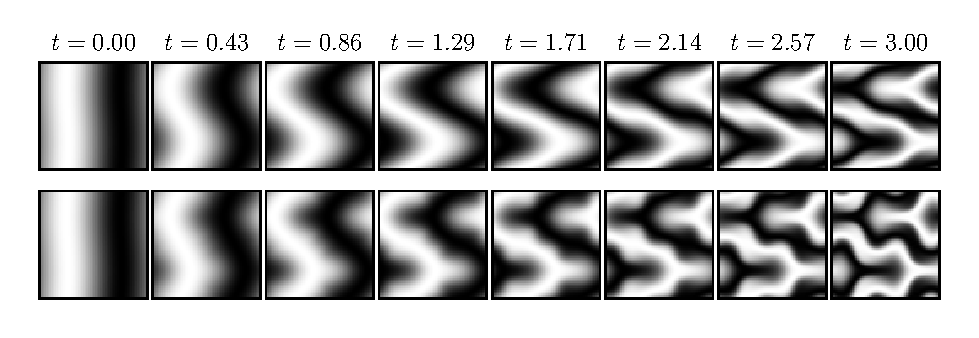
\includegraphics[width=\textwidth]{ch-git/images/output_N64_T3p0_gamma_1p0_kappa_0_L1p0/film.eps}
\caption{The top filmstrip is the local-in-time strategy while the bottom filmstrip is the global-in-time strategy. $\Gamma = 1.0$.}
\label{fig:lit_vs_git_film}
\end{figure}

\begin{figure}
\centering
\includegraphics[width=0.7\textwidth]{ch-git/images/output_N64_T3p0_gamma_1p0_kappa_0_L1p0/lit_vs_git_N64_T3p0_kappa0_L1_gamma1p0.eps}
\caption{The top subplot shows a comparison of local-in-time agains global-in-time optimization for fixed enstrophy ($\Gamma = 1.0$). The bottoms subplot shows uniform expenditure in time of the stirring budget as expected.}
\label{fig:lit_vs_git}
\end{figure}


\subsection{Comparison with local-in-time optimization}
We investigate the performance of global-in-time optimization relative to instantaneous optimization for $\Gamma =1.0$, $\kappa = 0$, $L=1.0$, $M=1000$, $N=64$ and $T=3.0$. We consider the performance of mixing the initial condition $\theta_0(\mathbf{x}) = \sin( 2\pi x/L).$ We use the numerical scheme described in section \ref{sec:target_method}. Python code is provided in Appendix \ref{app:git_code}. The resulting flow is shown in the bottom filmstrip of Figure \ref{fig:lit_vs_git_film} while the local-in-time flow is shown in the top filmstrip for comparison. Quantities of interests for this global-in-time optimal flow are shown in Figure \ref{fig:lit_vs_git}. The top subplot of Figure \ref{fig:lit_vs_git} shows how the $H^{-1}$ mix-norm varies in time. Note how initially the local-in-time flow outperforms the global-in-time optimal flow for short times, obviously due to the fact that it is a greedy algorithm maximizing mixing in the near future. However, note that the global-in-time flow eventually outperforms local-in-time by the final time as expected. Furthermore, observe that enstrophy is expended uniformly in time as expected by the previous analytical result.









